\chapter{Testing}
\label{chap:testing}
% https://docs.google.com/document/d/1yKFA3TraYr12bRBNZf6WqOU08AT3iYiavBPR_fY58NE/edit?usp=sharing

% % % %

\section{Vorgehen}
Jeder der folgenden Tests wurde vor der Umsetzung definiert.
Nach erfolgter Umsetzung wurden alle Tests durchgeführt.

Die Tests können in zwei Kategorien eingeteilt werden: in zustandsspezifische Tests (im \secref{sec:stateSpecificTest}) und in allgemeine Tests (im \secref{sec:generalTest}).

\section{Zustandsspezifische Tests}
\label{sec:stateSpecificTest}
\subsection{Off-Zustand (Z0)}
\subsubsection{T0.1 - Übergang zum Reset-Zustand (Z1)}
\begin{table}[H]
	\centering
	\small\renewcommand{\arraystretch}{1.4}
	\rowcolors{1}{tablerowcolor}{tablebodycolor}
	%
	\captionabove{Z0: T0.1}
	%
	\begin{tabularx}{0.9\textwidth}{ L{0.15\linewidth} | X  }%
		\hline
		Titel: & T0.3 - erfolgreiche Programm Initialisierung (Verbindung zu Leap Motion und Crazyflie)\\
		Status: & \textit{ok}\\
		Beschreibung: & Das System kann erfolgreich gestartet werden. Die Steuerung befindet sich anschliessend im \textit{Reset Zustand}.\\
		Ausgangslage: & Der Leap Motion und die Crazyflie sind korrekt verbunden, die notwendigen Services laufen und die Hardware ist eingeschaltet.\\
		Ergebnisse: & 30. August 2015: 
		Der Test war erfolgreich. Nach dem Verbinden der externen Geräten, wurde die Steuerung in den \textit{Reset-Zustand} versetzt.
		\\
		Massnahmen: & -\\
		\hline
	\end{tabularx}
\end{table}
\begin{figure}[H]
	\centering
	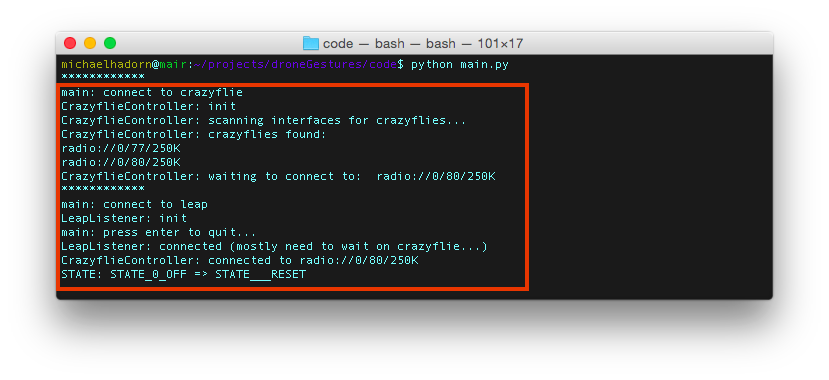
\includegraphics[width=1.0\textwidth]{images/testing/t0_1_success_edit.png}
	\caption{Konsolen-Output: T0.1 - Übergang zum Init Zustand (Z1)}
\end{figure}


\subsubsection{T0.2 - Verbindung zur Drohne ist fehlgeschlagen}
\begin{table}[H]
	\centering
	\small\renewcommand{\arraystretch}{1.4}
	\rowcolors{1}{tablerowcolor}{tablebodycolor}
	%
	\captionabove{Z0: T0.2}
	%
	\begin{tabularx}{0.9\textwidth}{ L{0.15\linewidth} | X  }%
		\hline
		Titel: & T0.2 - Verbindung zur Drohne ist fehlgeschlagen\\
		Status: & \textit{ok}\\
		Beschreibung: & Wenn bei der Initialisierung des Programmes, die Drohne nicht korrekt verbunden werden kann, soll die Steuerung nicht beginnen (ausser der Debug-Mode ist aktiv). Zudem soll eine Fehlermeldung ausgegeben werden. Beim abbrechen des Programmes, sollen alle Komponenten erfolgreich heruntergefahren werden.\\
		Ausgangslage: & -\\
		Ergebnisse: & 30. August 2015: 
		Der Test war erfolgreich. Die Steuerung wurde nicht gestartet. Die Fehlermeldung wurde ausgegeben. Beim Abbruch, wurden alle Komponenten heruntergefahren.
		\\
		Massnahmen: & -\\
		\hline
	\end{tabularx}
\end{table}
\begin{figure}[H]
	\centering
	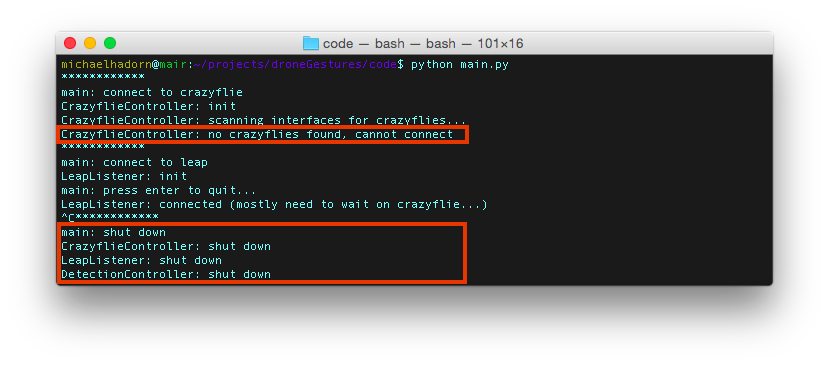
\includegraphics[width=1.0\textwidth]{images/testing/t0_2_no_drone_2_edit.png}
	\caption{Konsolen-Output: T0.2 - Verbindung zur Drohne ist fehlgeschlagen}
\end{figure}


\subsubsection{T0.3 - Verbindung zum Leap Motion ist fehlgeschlagen}
\begin{table}[H]
	\centering
	\small\renewcommand{\arraystretch}{1.4}
	\rowcolors{1}{tablerowcolor}{tablebodycolor}
	%
	\captionabove{Z0: T0.3}
	%
	\begin{tabularx}{0.9\textwidth}{ L{0.15\linewidth} | X  }%
		\hline
		Titel: & T0.3 - Verbindung zum Leap Motion ist fehlgeschlagen\\
		Status: & \textit{ok}\\
		Beschreibung: & Wenn bei der Initialisierung des Programmes, der Leap Motion nicht korrekt verbunden werden kann, soll die Steuerung nicht beginnen.
		Beim Abbrechen des Programmes, sollen alle Komponenten erfolgreich heruntergefahren werden.\\
		Ausgangslage: & -\\
		Ergebnisse: & 30. August 2015: 
		Der Test war erfolgreich. Beim Abbruch, wurden alle Komponenten heruntergefahren.
		\\
		Massnahmen: & -\\
		\hline
	\end{tabularx}
\end{table}


% % % %

\subsection{Init-Zustand (Z1) inkl. Reset}

\subsubsection{T1.1 - Übergang zum Flugbereiten Zustand (Z2)}
\begin{table}[H]
	\centering
	\small\renewcommand{\arraystretch}{1.4}
	\rowcolors{1}{tablerowcolor}{tablebodycolor}
	%
	\captionabove{Z1: T1.1}
	%
	\begin{tabularx}{0.9\textwidth}{ L{0.15\linewidth} | X  }%
		\hline
		Titel: & T1.1 - Übergang zum \textit{Flugbereiten Zustand (Z2)}\\
		Status: & \textit{ok}\\
		Beschreibung: &  Um die Steuerung in den \textit{Flugbereiten Zustand (Z2)} zu versetzen, müssen folgende Gesten erkannt werden:
		\begin{itemize}
			\item offene und geschlossene Hand
			\item mind. 2 Sek. eine Faust
		\end{itemize}
		Anschliessend soll der Zustandswechsel erfolgen.
		\\
		Ausgangslage: & Die Steuerung muss sich im \textit{Init-Zustand (Z1)} befinden.\\
		Ergebnisse: & 30. August 2015: 
		Die Steuerung wurde korrekt in den \textit{Flugbereiten Zustand (Z2)} gesetzt.
		\\
		Massnahmen: & -\\
		\hline
	\end{tabularx}
\end{table}
\begin{figure}[H]
	\centering
	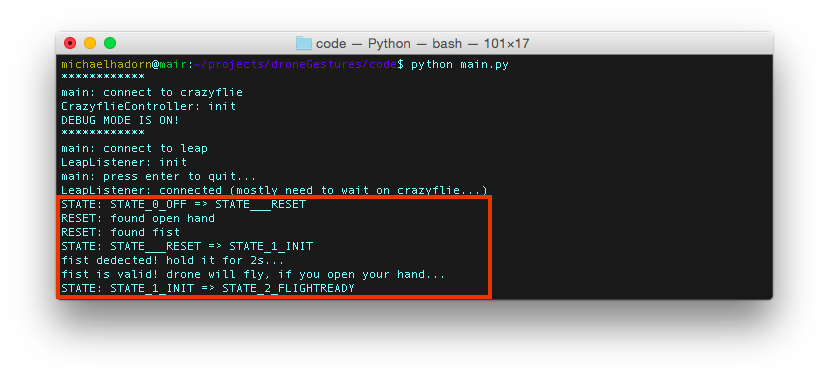
\includegraphics[width=1.0\textwidth]{images/testing/t1_1_succes_state_2_edit.png}
	\caption{Konsolen-Output: T1.1 - Übergang zum Flugbereiten Zustand (Z2)}
\end{figure}


% % % %

\subsection{Flugbereiten Zustand (Z2)}
\subsubsection{T2.1 - Übergang in Flug-Zustand (Z3)}
\begin{table}[H]
	\centering
	\small\renewcommand{\arraystretch}{1.4}
	\rowcolors{1}{tablerowcolor}{tablebodycolor}
	%
	\captionabove{Z2: T2.1}
	%
	\begin{tabularx}{0.9\textwidth}{ L{0.15\linewidth} | X  }%
		\hline
		Titel: & T2.1 - Übergang in \textit{Flug-Zustand (Z3)}\\
		Status: & \textit{ok}\\
		Beschreibung: &  Wird eine offene Hand erkannt, wird die Höhe der Hand Null-Referenz der Höhe verwendet.
		\\
		Ausgangslage: & Die Steuerung muss sich im \textit{Flugbereiten Zustand (Z2)} befinden.\\
		Ergebnisse: & 30. August 2015: 
		Funktioniert.
		\\
		Massnahmen: & -\\
		\hline
	\end{tabularx}
\end{table}
\begin{figure}[H]
	\centering
	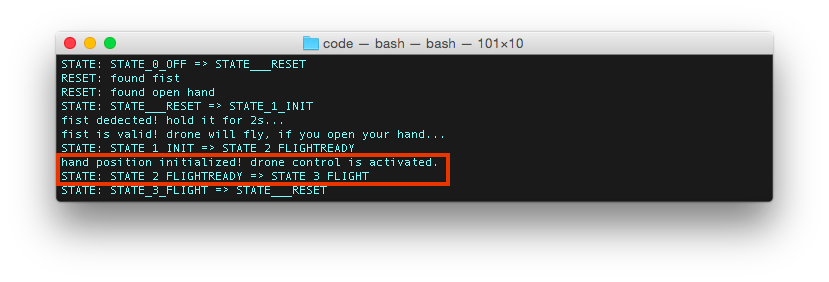
\includegraphics[width=1.0\textwidth]{images/testing/t2_1_success_state_3.png}
	\caption{Konsolen-Output: T2.1 - Übergang in Flug-Zustand (Z3)}
\end{figure}


\subsubsection{T2.2 - Offene Hand auf ungültiger Höhe erkannt}
\begin{table}[H]
	\centering
	\small\renewcommand{\arraystretch}{1.4}
	\rowcolors{1}{tablerowcolor}{tablebodycolor}
	%
	\captionabove{Z2: T2.2}
	%
	\begin{tabularx}{0.9\textwidth}{ L{0.15\linewidth} | X  }%
		\hline
		Titel: & Offene Hand auf ungültiger Höhe erkannt\\
		Status: & \textit{ok}\\
		Beschreibung: &  
		Wird die Hand auf einer ungültigen Höhe (nicht innerhalb 10 -- 35 cm über dem Sensor) erkannt, soll eine Meldung ausgegeben werden und in den \textit{Reset-Zustand} gewechselt werden.
		\\
		Ausgangslage: & Die Steuerung muss sich im \textit{Flugbereiten Zustand (Z2)} befinden.\\
		Ergebnisse: & 30. August 2015: 
		Funktioniert.
		\\
		Massnahmen: & -\\
		\hline
	\end{tabularx}
\end{table}
\begin{figure}[H]
	\centering
	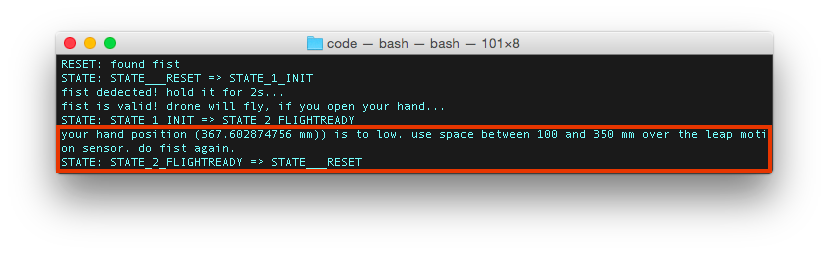
\includegraphics[width=1.0\textwidth]{images/testing/t2_2_invalid_height_edit.png}
	\caption{Konsolen-Output: T2.2 - Übergang in Flug-Zustand (Z3)}
\end{figure}



% % % %

\subsection{Flug-Zustand (Z3)}
\subsubsection{T3.1 - Kontrollierter Flugabbruch / Übergang in Reset-Zustand}
\begin{table}[H]
	\centering
	\small\renewcommand{\arraystretch}{1.4}
	\rowcolors{1}{tablerowcolor}{tablebodycolor}
	%
	\captionabove{Z3: T3.1}
	%
	\begin{tabularx}{0.9\textwidth}{ L{0.15\linewidth} | X  }%
		\hline
		Titel: & T3.1 - Kontrollierter Flugabbruch / Übergang in Reset-Zustand\\
		Status: & \textit{ok}\\
		Beschreibung: &  
		Wird im Flug eine Faust erkannt, soll sofort in den Reset-Zustand gewechselt werden.
		\\
		Ausgangslage: & Die Steuerung muss sich im \textit{Flug-Zustand (Z3)} befinden.\\
		Ergebnisse: & 30. August 2015: 
		Funktioniert.
		\\
		Massnahmen: & -\\
		\hline
	\end{tabularx}
\end{table}
\begin{figure}[H]
	\centering
	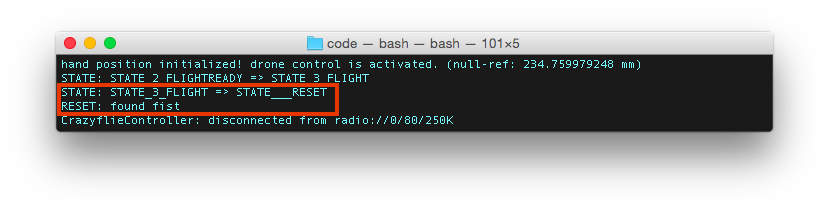
\includegraphics[width=1.0\textwidth]{images/testing/t3_1_success_state_reset_edit.png}
	\caption{Konsolen-Output: T3.1 - T3.1 - Kontrollierter Flugabbruch / Übergang in Reset-Zustand}
\end{figure}


\subsubsection{T3.2 - No-Thrust Zone}
\begin{table}[H]
	\centering
	\small\renewcommand{\arraystretch}{1.4}
	\rowcolors{1}{tablerowcolor}{tablebodycolor}
	%
	\captionabove{Z3: T3.2}
	%
	\begin{tabularx}{0.9\textwidth}{ L{0.15\linewidth} | X  }%
		\hline
		Titel: & T3.2 - No-Thrust Zone\\
		Status: & \textit{ok}\\
		Beschreibung: &  
		Nachdem die Steuerung initialisiert wurde und die relative Höhe der offenen Hand gemessen wurde, soll eine zusätzliche Schutzzone (2\,cm) in der noch kein Thrust gesendet wird, erzeugt werden.
		Erst wenn sich die Hand höher als die Schutzzone befindet, soll die Drohne losfliegen.
		\\
		Ausgangslage: & Die Steuerung muss sich im \textit{Flug-Zustand (Z3)} befinden.\\
		Ergebnisse: & 30. August 2015: 
		Funktioniert.
		\\
		Massnahmen: & -\\
		\hline
	\end{tabularx}
\end{table}



% % % %

\section{Allgemeine Tests}
\label{sec:generalTest}
\subsection{Allgemeines Verhalten}
\subsubsection{TA.1 - Mehrere Hände erkannt oder Hand verloren}
\begin{table}[H]
	\centering
	\small\renewcommand{\arraystretch}{1.4}
	\rowcolors{1}{tablerowcolor}{tablebodycolor}
	%
	\captionabove{A: TA.1}
	%
	\begin{tabularx}{0.9\textwidth}{ L{0.15\linewidth} | X  }%
		\hline
		Titel: & TA.1 - Mehrere Hände erkannt oder Hand verloren\\
		Status: & \textit{ok}\\
		Beschreibung: &  Sobald mehrere Hände erkennt werden oder keine Hand mehr erkannt wird, soll in den \textit{Reset-Zustand} gewechselt werden.\\
		Ausgangslage: & Programm wurde erfolgreich initialisiert. Es spielt keine Rolle in welchem Zustand sich die Steuerung befindet.\\
		Ergebnisse: & 30. August 2015: 
		Sobald mehr als eine Hand erkannt wird oder die Hand verloren geht, wird sofort in den \textit{Reset-Zustand} gewechselt.
		\\
		Massnahmen: & -\\
		\hline
	\end{tabularx}
\end{table}
\begin{figure}[H]
	\centering
	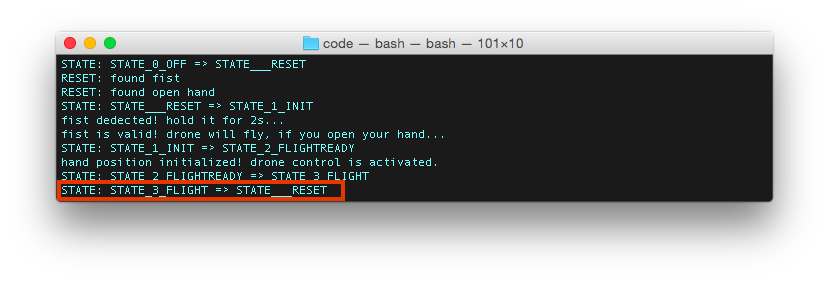
\includegraphics[width=1.0\textwidth]{images/testing/ta_1_lost_multi_hand_2_edit.png}
	\caption{TA.1 - Mehrere Hände erkannt oder Hand verloren}
\end{figure}


\subsubsection{TA.2 - Verbindungsunterbruch zur Drohne}
\begin{table}[H]
	\centering
	\small\renewcommand{\arraystretch}{1.4}
	\rowcolors{1}{tablerowcolor}{tablebodycolor}
	%
	\captionabove{A: TA.2}
	%
	\begin{tabularx}{0.9\textwidth}{ L{0.15\linewidth} | X  }%
		\hline
		Titel: & TA.2 - Verbindungsunterbruch zur Drohne\\
		Status: & \textit{ok}\\
		Beschreibung: &  Falls die Verbindung zur Drohne abbricht, soll die Steuerung in den \textit{Off-Zustand (Z0)} versetzt werden.
		Eine Meldung soll ausgegeben werden.
		Anschliessend kann das Programm beendet und bei Bedarf neu gestartet werden.
		\\
		Ausgangslage: & Die Verbindung zur Drohne wurde hergestellt. Es spielt keine Rolle in welchem Zustand sich die Steuerung befindet.\\
		Ergebnisse: & 30. August 2015: 
		Die Steuerung wird erfolgreich in den \textit{Off-Zustand (Z0)} versetzt.
		\\
		Massnahmen: & -\\
		\hline
	\end{tabularx}
\end{table}
\begin{figure}[H]
	\centering
	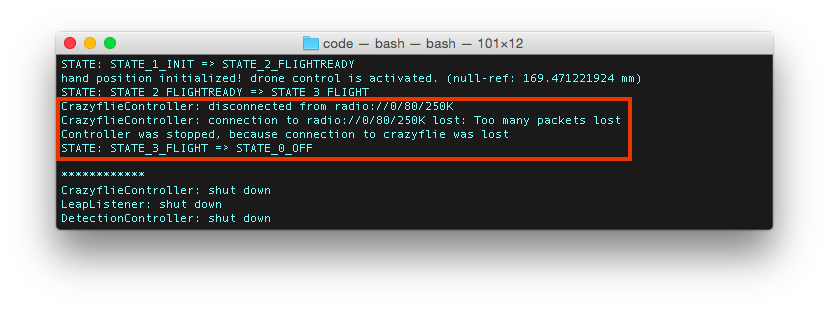
\includegraphics[width=1.0\textwidth]{images/testing/ta_2_disconnect_drone_edit.png}
	\caption{TA.2 - Mehrere Hände erkannt oder Hand verloren}
\end{figure}

